\documentclass[zihao=-4]{ctexart}
\usepackage[normalem]{ulem}
\useunder{\uline}{\ul}{}
%********************导言区宏包引入********************
\usepackage{xeCJK}
\usepackage{amssymb}
\usepackage{amsmath}
\usepackage{listings} %代码
\usepackage{graphicx}
\usepackage{multicol} %回车换段
\usepackage{xcolor}
\usepackage{geometry} %页面设置
\usepackage{fontspec}
\usepackage{setspace}
\usepackage{times}
\usepackage{fancyhdr} %页眉页脚
\pagestyle{fancy}
\usepackage{float} %表格位置
\usepackage{titlesec} %设置
\usepackage{titletoc}
\usepackage{ctex}
\usepackage{gbt7714}    %控制参考文献格式为国标
\usepackage{multirow}
\usepackage{booktabs}   %表格相关
\usepackage{setspace}   %设置行距
\usepackage{caption} %caption
\usepackage{subcaption} %子图的caption
\usepackage{changepage} %左右缩进


\graphicspath{ {pictures/} }
\let\algorithm\relax
\let\endalgorithm\relax
\usepackage[ruled,vlined]{algorithm2e}%[ruled,vlined]{
\usepackage{algpseudocode}
\renewcommand{\algorithmicrequire}{\textbf{Input:}} 
\renewcommand{\algorithmicensure}{\textbf{Output:}}
%\renewcommand\thepage{\zihao{-5} ~\arabic{page}~}%页码字号

%定义两个arg
\DeclareMathOperator*{\argmax}{arg\,max}
\DeclareMathOperator*{\argmin}{arg\,min}
\DeclareCaptionLabelSeparator{mysep}{\space\space}  %自定义caption格式
\captionsetup[figure]{font={small}, labelfont=bf, labelsep=mysep, textfont=bf}   %图片caption格式
\captionsetup[table]{font={small}, labelfont=bf, labelsep=mysep, textfont={bf}}   %表格caption格式
\bibliographystyle{gbt7714-numerical} %修改了title斜体内容

%********************导言区宏包引入********************
%********************第三方字体引入********************
%\setCJKmainfont[Path=fonts/,BoldFont=simhei.ttf,ItalicFont=simkai.ttf,SlantedFont=simfang.ttf]{simsun.ttc}
%中文字体涵盖黑体、宋体、楷体、仿宋
\setmainfont[Path=fonts/, 
BoldFont = times-new-roman-bold.ttf,
ItalicFont = times-new-roman-italic.ttf,
BoldItalicFont = times-new-roman-bold-italic.ttf
]{times-new-roman.ttf}
\setmonofont[Path=fonts/]{Courier New.ttf}
\setCJKfamilyfont{hwzs}[Path=fonts/]{STKzhongsong.ttf}%使用STZhogsong华文中宋字体
\newcommand{\zhongsong}{\CJKfamily{hwzs}}
\setCJKfamilyfont{hwxw}[Path=fonts/]{STKxinwei.ttf} % XSP 2023/3/3:
\newcommand{\xinwei}{\CJKfamily{hwxw}}              %  使用STZxinwei华文新魏字体.

%********************第三方字体引入********************

%********************代码段设置********************
% by yjw
% \texttt 用于行内代码,等宽字体,不知道让不让用
\usepackage{listings} % 用于代码排版
\usepackage{xcolor} % 用于代码高亮

% 定义代码块样式
\lstdefinestyle{codeblock}{
    backgroundcolor=\color{white},    % 背景颜色
    basicstyle=\ttfamily\small,       % 设置字体样式
    breakatwhitespace=false,          % 是否只在空白处自动断行
    breaklines=true,                  % 自动断行
    captionpos=b,                     % 标题位置
    commentstyle=\color{gray},       % 注释风格
    frame=single,                     % 单框
    keepspaces=true,                  % 保持空格
    keywordstyle=\color{blue},        % 关键字风格
    numbers=left,                     % 行号位置
    numbersep=8pt,                    % 行号与代码的距离
    numberstyle=\tiny\color{gray},    % 行号样式
    rulecolor=\color{black},          % 框架颜色
    showspaces=false,                 % 不显示空格
    showstringspaces=false,           % 字符串中不显示空格
    showtabs=false,                   % 不显示制表符
    stepnumber=1,                     % 步长
    stringstyle=\color{orange},       % 字符串风格
    tabsize=2,                        % 制表符占用空格数
    xleftmargin=\parindent,           % 左边距
    framexleftmargin=12pt,             % 框架左边距,增加些许间距以包含行号
}
\lstset{style=codeblock}

\usepackage{hyperref} %超链接支持
%********************代码段设置********************

%********************中文字号设置********************
%\newcommand{\chuhao}{\fontsize{42pt}{\baselineskip}\selectfont}
\newcommand{\chuhao}{\fontsize{42pt}{0}}
\newcommand{\xiaochu}{\fontsize{36pt}{0}}
\newcommand{\yihao}{\fontsize{28pt}{0}}
\newcommand{\erhao}{\fontsize{21pt}{0}}
\newcommand{\xiaoer}{\fontsize{18pt}{0}}
\newcommand{\sanhao}{\fontsize{16pt}{0}}
\newcommand{\sihao}{\fontsize{14pt}{0}}
\newcommand{\xiaosi}{\fontsize{12pt}{0}}
\newcommand{\wuhao}{\fontsize{10.5pt}{0}}
\newcommand{\xiaowu}{\fontsize{9pt}{0}}
\newcommand{\liuhao}{\fontsize{8pt}{0}}
\newcommand{\qihao}{\fontsize{5.25pt}{0}}
%********************中文字号设置********************


%********************页边距设置********************
\geometry{left=3cm,right=2cm,top=2.5cm,bottom=2.5cm}
\geometry{a4paper} % xsp 2023/3/7: 调整纸张大小为A4
%********************页边距设置********************

%********************段间距设置********************
\newcommand{\setParDis}{\setlength {\parskip} {0pt} }
%请在每部分使用这个
%********************段间距设置********************

%********************子文件导入区域****************
% 用于仅编译部分导入文件
% \includeonly{subtexs/ros_background, }

\begin{document}
%********************页眉页脚设置********************
\lhead{}%设置左页眉为空
\rhead{}%设置左页眉为空
\setlength{\headwidth}{\textwidth}% 2023/3/3 XSP: 页眉长度适应文本
%********************页眉页脚设置********************


%********************标题格式设置********************

%\setcounter{secnumdepth}{0}%该命令取消了章标题前数字label

\CTEXsetup[name={,、},number={\chinese{section}}]{section}
\CTEXsetup[name={(,)},number={\chinese{subsection}}]{subsection}
\CTEXsetup[name={,.},number={\arabic{subsubsection}}]{subsubsection}% 不加会导致目录格式错误
% 设置subsubsection等格式
% \titleformat{\section}[block]{\sanhao\bfseries\centering}{\chinese{section}、}{0pt}{}[]
% \titleformat{\subsection}[block]{\sihao\bfseries}{(\chinese{subsection})}{0pt}{}[]
% \titleformat{\subsubsection}[block]{\xiaosi\bfseries}{\arabic{subsubsection}、}{0pt}{}[]
\titleformat{\section}[block]{\sanhao\heiti\centering}{\chinese{section}、}{0pt}{}[]    % XSP 2023/3/3:
\titleformat{\subsection}[block]{\sihao\heiti}{(\chinese{subsection})}{0pt}{}[]       %   将正文标题字体由加粗
\titleformat{\subsubsection}[block]{\xiaosi\heiti}{\arabic{subsubsection}.}{0pt}{}[]   % 修改为黑体。
\titlespacing{\section}{0pt}{25pt}{12pt}
\titlespacing{\subsection}{0pt}{7pt}{7pt}
\titlespacing{\subsubsection}{0pt}{5pt}{4pt}

\titlecontents{section}[1.6em]{\addvspace{2pt}\filright}
{\contentspush{\thecontentslabel\hspace{0.8em}}}
{}{\titlerule*[8pt]{.}\contentspage}

\titlecontents{subsection}[3.2em]{\addvspace{2pt}\filright}
{\contentspush{\thecontentslabel\hspace{0.8em}}}
{}{\titlerule*[8pt]{.}\contentspage}

\titlecontents{subsubsection}[6.4em]{\addvspace{2pt}\filright}
{\contentspush{\thecontentslabel\hspace{0.8em}}}
{}{\titlerule*[8pt]{.}\contentspage}
%********************标题格式设置********************

%\setcounter{section}{-3}  %标题计数器
%\stepcounter{section}

%*******************行间距段前段后*******************
\linespread{1.8}
%行间距为实际行间距乘以1.2,如此处实际为1.5倍行距
\setlength{\parskip}{0.5\baselineskip}
%*******************行间距段前段后*******************



%********************封面部分********************
%
%     论文题目:应准确、鲜明、简洁,能概括整个论文中最主要和最重要的内容。
% 题目不超过20个中文字,若语意未尽,可用副标题补充说明。副标题应处于从属
% 地位,一般可在题目的下一行用破折号“——”引出。论文题目应避免使用不常用缩
% 略词、首字母缩写字、字符、代号和公式等。
%
\def\Fengru{第三十四届“冯如杯”竞赛主赛道}
\leftline{
\includegraphics[scale=1]{pictures/xiaohui.png}} % XSP 2023/3/3: 取消校徽段首缩进
%格式控制部分
% \par \  
% \par \
% \par \
\vspace{32pt}
\begin{center}

\includegraphics[height=2.25cm, width=12.78cm, scale=1]{pictures/xiaoming.png}
\end{center}
%格式控制部分
\vspace{12pt}

\begin{spacing}{3}
    % \erhao
    \begin{center}
      {
        \fontsize{22pt}{3}\selectfont
        \zhongsong{\Fengru 项目论文Latex模板} %黑体这样调用,其余字体同理
      } 
        % \zhongsong{“冯如杯”竞赛主赛道项目是什么}
    \end{center}
    \rightline{\xinwei\sanhao{——基于 Latex 的论文模板}} % XSP 2023/3/3: 副标题二号华文新魏居右
\end{spacing}
%格式控制部分
% \par \ 
% \par \
\par \ 
\par \
\par \ 
\par \
% \begin{center}
%     \sihao
%     \textbf{学院:计算机学院}
%     \par \ 
%     \textbf{本模板原作者:Someday}
% \end{center}

%格式控制部分
\par \ 
\begin{center}
\sanhao
\centerline{\heiti{}}%封面年月去掉
\end{center}

\pagenumbering{gobble} %封面无页码
%\thispagestyle{empty}


\renewcommand{\headrulewidth}{0pt}%没有页眉装饰线
\clearpage
\pagenumbering{roman} %摘要目录页小写罗马

\xiaosi
\section*{摘要}
\begin{spacing}{1.5}
  \setParDis %设置段间距为 0
  本Latex模板是北京航空航天大学大学\Fengru 论文模板, 由北京航空航天大学校团委
基于GitHub用户\textbf{\textit{Somedaywilldo}}与\textbf{\textit{cpfy}}的成果迭代
开发而来。在此由衷感谢所有开发者对本模板的贡献与对“冯如杯”竞赛的大力支持。

摘要内容包括:“摘要”字样,摘要正文,关键词。在摘要的最下方另起一行,用显著的字符注明文本的关键词。

摘要是论文内容的简短陈述,应体现论文工作的核心思想。摘要一般约500字。摘要内容应涉及本项科研工作的目的和意义、研究思想和方法、研究成果和结论。

关键词是为用户查找文献,从文中选取出来用来揭示全文主题内容的一组词语或术语,应尽量采用词表中的规范词(参照相应的技术术语标准)。关键词一般为3到8个,按词条的外延层次排列。关键词之间用逗号分开,最后一个关键词后不打标点符号。

\end{spacing}
    
\textbf{关键词:}模糊测试技术,机器人操作系统,并发漏洞检测,内存安全漏洞检测,关键词5

\newpage
\section*{\textbf{Abstract}} % XSP 2023/3/8: Abstract 加粗
\begin{spacing}{1.5}
\begin{adjustwidth}{0.42cm}{0.42cm}
  \setParDis %设置段间距为 0

\qquad This Latex template for the 33rd Fengru Cup Competition of 
Beihang University, is developed by Communist Youth League Committee of BUAA 
iteratively based on the contribution of GitHub 
users \textbf{\textit{Somedaywilldo}} and \textbf{\textit{cpfy}}. 
Here, we would like to thank all the developers for their 
contributions to this template and for their support of the Fengru Cup Competition.

The abstract includes: the word "Abstract", the body of the abstract, and the keywords. On a separate line at the bottom of the abstract, indicate the key words of the text in prominent characters.

The abstract is a short statement of the content of the paper and should reflect the core ideas of the paper work. The abstract is usually about 500 words. The abstract should cover the purpose and significance of this scientific work, research ideas and methods, research results and conclusions.

Keywords are a set of words or terms selected from the text to reveal the subject content of the whole text for the user to find the literature, and the standardized words in the word list (refer to the corresponding technical terminology standards) should be used as much as possible. The keywords are usually 3 to 8, arranged according to the level of extensibility of the words. The keywords are separated by commas, and no punctuation marks are used after the last keyword.

\textbf{Keywords: Keywords 1, Keywords 2, Keywords 3, Keywords 5, Keywords 6}
\end{adjustwidth}
\end{spacing}



%********************摘要部分********************


%********************目录部分********************
\clearpage
\tableofcontents
\clearpage
%********************目录部分********************



\renewcommand{\headrulewidth}{0.4pt} %恢复页眉装饰线

%********************正文页眉部分********************
%\lhead{} 
\chead{\xiaowu 北京航空航天大学\Fengru 参赛作品} %设置居中页眉
%********************正文页眉部分********************

\pagenumbering{arabic} %正文页码从1开始,用阿拉伯数字
\setcounter{page}{1} 

%%%%%%%%%%%%%%%%%%%%%% 一 作品概述
\section{作品概述}
  \setParDis %设置段间距为 0
\begin{spacing}{1.5} % 行距1.5


\subsection{背景介绍}
\setParDis %设置段间距为 0
%@author: lhy
% \subsection{背景介绍}
%@author: lhy
\subsubsection{ROS系统重要性}
人类生活与机器人密不可分。传统上,机器人在农业和制造业中被广泛用于任务自动化。最近的发展让机器人更加贴近每个人的日常生活。例如,亚马逊和谷歌正在部署无人配送系统[22,23],使用无人驾驶飞行器,机器人吸尘器的市场规模年增长率达到23\%[24],以及在2012年到2018年间,使用机器人进行手术的比例从2\%增加到15\%[25],显示出机器人产业为适应人类需求而快速增长的态势。同时,现代机器人,如自动驾驶车辆,正在变得更加复杂,要求集成复杂的子系统,例如感知、感觉、规划和执行。

为了应对开发复杂机器人系统的更高需求,机器人操作系统(ROS)[1]正在获得越来越多的关注。ROS是一个开源的中间件套件,用于机器人开发,它具有分布式机器人进程的消息传递机制、硬件抽象、广泛的开发工具(例如,模拟器)和机器人库(例如,路径规划算法)。使用ROS,开发者可以加速开发过程,无需重新发明轮子,而是可以专注于他们机器人的核心功能。凭借其多语言和多平台支持的理念,ROS正在成为机器人编程中的实际标准;它已被广泛采用于工业[26,27]、军事[28,29]、研究机构以及个人,预计到2024年将为55\%的商业机器人提供动力[30]。近些年ROS系统相关论文数量与Wiki用户数量如图1所示:

\begin{figure}[H]
  \centering
  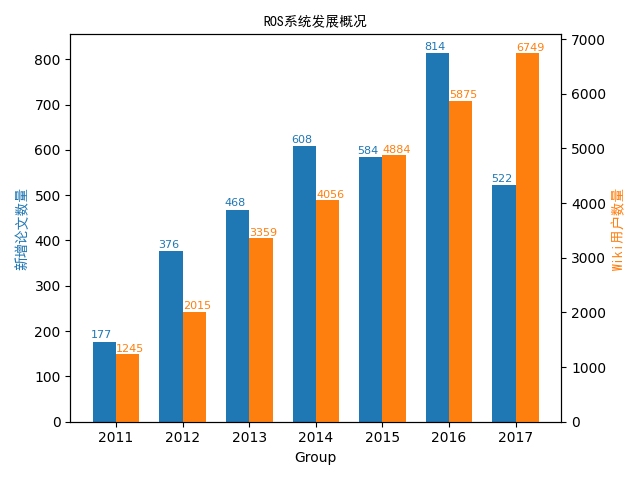
\includegraphics[width=0.8\textwidth]{ros_papers.png}
  \caption{ROS系统相关论文数量与Wiki用户数量}
\end{figure}

机器人操作系统(ROS)是一个开源平台,它为用C++和Python等不同语言实现机器人软件提供了许多实用的工具和库。超过740家商业公司正在使用ROS[2]来开发数百种实际应用的机器人[3],这表明了其在机器人开发中的流行度。然而,开发可靠的ROS程序具有挑战性,因为机器人可以在复杂的物理环境中工作,并可能遇到各种异常情况(如无效的配置参数和异常的传感器信息)。如果ROS程序不够可靠,它们的错误可能在与人类和其他机器人交互时导致危险事故。

ROS本身的缺陷或者开发者在应用中常用的ROS使用方式可能会影响依赖于ROS的广泛机器人系统,并对许多用户的安全和保障造成严重破坏。例如,ROS版本1没有认证的概念,允许网络上的任何实体完全访问任何机器人系统,窃听内部消息,甚至在知道IP地址和端口的情况下劫持执行。实际上,在互联网上扫描默认的ROS端口两个月后[31],发现部署在28个国家的超过100个ROS系统,这些系统完全暴露于此类攻击之下。ROS的最新版本(即ROS 2)在设计和实现时考虑了这些问题,并邀请了更广泛的公众对安全性进行审查。不幸的是,现有的工作和解决方案要么专注于关于认证和授权方法的网络安全方面[32,33,34,35],要么专注于回归测试[36],使得ROS社区在寻找影响机器人系统的健壮性和正确性的未知错误方面缺乏一种系统的测试方法。
\subsubsection{自动驾驶兴起与ROS}
自动驾驶技术的兴起标志着交通运输领域的一次重大革命,其不仅预示着交通安全、效率和环境影响的根本改进,而且还预示着个人出行和货物运输方式的深刻变革,而这一过程在很大程度上得益于机器人操作系统(Robot Operating System,ROS)的发展和应用。近年来,由于计算能力的显著提升、大数据技术的发展、人工智能算法的进步以及传感器技术的优化,自动驾驶汽车从理论研究和小规模试验逐步走向了公路测试和商业化应用的初步阶段。

根据国际汽车工程师学会(SAE)的定义[1],自动驾驶分为六个级别,从0级(无自动化)到5级(完全自动化)。目前,多数公开测试和部分商业化应用的自动驾驶汽车处于3级(有条件自动化)到4级(高度自动化)。尽管完全自动化(5级)的汽车尚未广泛部署,但多个技术开发者和制造商已经在进行相关的研发工作,并在不同国家和地区开展了路试。

随着自动驾驶技术的进步,对处理大量传感器数据、实现复杂决策逻辑和执行精确控制的需求不断增加,ROS的可扩展性和灵活性在此过程中显示出其不可或缺的价值。例如,ROS的消息传递系统支持多种编程语言,允许异构系统高效集成。此外,其庞大的开源社区贡献了大量的软件包,覆盖从3D视觉到路径规划等各种功能,极大地丰富了自动驾驶汽车的研发资源库。

经济学人智库的一份报告预测[2],到2035年,全球自动驾驶汽车的数量将达到近7500万辆。而麦肯锡公司的一项研究则估计[3],自动驾驶技术的全面部署将使交通事故造成的死亡人数减少90\%,同时还将大幅度提升道路运输效率和减少碳排放。图2展示了PRECEDENCE RESEARCH机构预测的未来自动驾驶市场规模:

\begin{figure}[H]
  \centering
  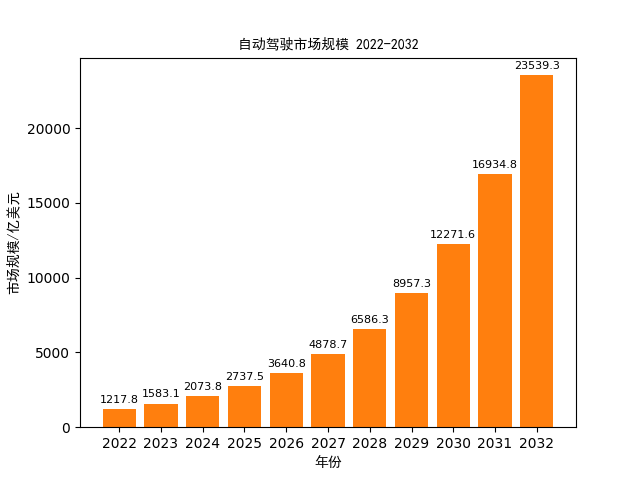
\includegraphics[width=0.8\textwidth]{market_size.png}
  \caption{自动驾驶市场规模}
  \label{fig:my_label}
\end{figure}

尽管自动驾驶技术的前景被广泛看好,但其商业化应用和普及还面临多重挑战,包括技术完善度、法律法规、道德伦理、消费者接受度以及基础设施配套等。例如,自动驾驶汽车在复杂的城市交通环境中的表现,以及在极端天气条件下的可靠性,仍然是技术研发中的重要挑战。

未来,随着相关技术的进一步成熟和相关政策的完善,自动驾驶汽车有望在更广泛的领域得到应用,从而实现对交通系统的根本性改造和优化。这将不仅影响交通运输本身,还将对城市规划、能源消费、环境保护以及人们的生活方式产生深远影响。

\subsubsection{自动驾驶产生漏洞的危害}
尽管自动驾驶汽车(AVs)承诺通过减少人为错误来增加道路安全,它们固有的技术漏洞却可能导致严重的安全后果。据国家公路交通安全管理局(NHTSA)估计,94\%的严重交通事故是由人为因素引起的,而自动驾驶技术的开发者们宣称,通过消除这一因素,可以极大地提高道路安全性[4]。然而,这种安全性的提升假设基于自动驾驶系统能够无缺陷地执行其预定任务,这在实践中往往难以实现。

自动驾驶汽车的技术漏洞主要分为两类:软件漏洞和硬件故障。软件漏洞包括但不限于算法错误、安全漏洞以及对异常情况的处理不足。硬件故障可能涉及传感器故障、执行机构的故障或其他关键组件的损坏。这些技术漏洞不仅可能导致单一车辆的操作失败,还可能对整个交通系统产生连锁反应,特别是在高度自动化和互联的交通环境中。

例如,2018年3月,在美国亚利桑那州发生了一起致命的自动驾驶汽车事故,一名行人在穿越街道时被一辆自动模式下的Uber汽车撞击,导致死亡。初步调查显示,该事故部分原因是系统无法正确识别并响应行人[5]。这一事件凸显了即使在自动驾驶技术取得显著进步的情况下,技术漏洞仍然可能导致灾难性后果。

此外,安全研究人员已经证明,自动驾驶汽车系统的安全漏洞可以被黑客利用,进而控制车辆的行驶方向或速度,造成严重安全威胁[6]。例如,通过篡改车辆的环境感知系统接收到的数据,攻击者可以使汽车忽略停车标志或其他关键交通信号,导致交通事故。

综上所述,尽管自动驾驶技术的发展被寄予厚望,能够在根本上改变我们的交通系统,降低事故率,提高交通效率,但技术漏洞的存在表明,要实现这些目标,还需要克服重大的技术和安全挑战。这要求汽车制造商、技术开发者、立法者和监管机构合作,不断提高自动驾驶系统的安全性和可靠性,同时为可能出现的技术漏洞和安全威胁制定全面的应对策略。



\subsection{研究现状}
\setParDis %设置段间距为 0
\subsubsection{ROS常见测试方案}
%@author: yjw
普通单元测试, 代码分析工具
\subsubsection{模糊测试及其应用}
%@author: jfb
强调:模糊测试目前很火,但是没有用到ros上

\subsection{作品概述}
\setParDis %设置段间距为 0
%@author: yjw


%%%%%%%%%%%%%%%%%%%%%% 二 作品设计与实现
\section{作品设计与实现}
\setParDis %设置段间距为 0

\subsection{技术背景与预备知识}
\setParDis %设置段间距为 0
%@author: jfb
\subsubsection{模糊测试框架}
\subsubsection{漏洞种类及危害}
%@author: wkt
\subsubsection{ASan}
\subsubsection{基于覆盖率的遗传算法}
\subsubsection{ROS机制}
%author: yjw, 2024-4-1

在 ROS 2的体系结构中,节点(Node)是最基本的执行单位,负责特定功能的实现,如数据处理或硬件接口。
每个节点可以包含多种通信机制,包括订阅者(Topic Subscribers)、定时器(Timer)、服务服务器(Service Servers)
和服务客户端(Service Clients),如图\ref{pic:rns}。这些通信实体的目的是为了接收和发送数据,以及提供不同的服务。

节点注册到执行器(Executor)中,执行器是一个控制实体,负责协调节点的活动。
当节点的一个通信事件发生时,比如收到一个主题消息或服务请求,执行器会调用相应的处理函数,或称为回调函数(Callback)。
这些回调函数是预先定义的,用来响应特定类型的事件,如 \texttt{topic\_receive()} 用于处理主题消息,
\texttt{request\_receive()}用于处理服务请求,\texttt{time\_up()}用于处理定时器完成计时。

在节点的生命周期中,可以使用生命周期状态机(Lifecycle SM)来管理节点的状态,这在管理复杂节点时特别有用。
生命周期状态机允许节点在不同状态之间转换,如激活(activate)、去激活(deactivate)和清理(cleanup)。
每个状态变化都可以有对应的回调函数,例如\texttt{setting()}在节点激活时调用,用于声明节点接口、
节点执行器(Executor)、通信订阅和服务订阅等一系列节点功能实体;\texttt{activate()} 用于节点初始化完毕开始服务,
此时节点处于正常工作状态; \texttt{cleanup()}在节点清理资源时调用,用于释放节点所持有的微机资源。

\textbf{ROS事件处理机制}: 

节点调用 \texttt{spin()} 函数来持续检查和处理事件,如伪代码\ref{lst:ros_spin}。

\begin{lstlisting}[language=Python, caption=ROS2事件循环示例, label=lst:ros_spin]
spin():
    while True:
        new_msg <- ros_dds_listener()
        handler <- get_callback(new_msg)
        Executor.execute(*handler)
        sleep(0.1)
\end{lstlisting}

\texttt{spin()} 实质是一种事件循环,它会保持节点循环和监听,检查系统中是否有新的ROS消息或待处理的消息,获取到消息实体后,
根据消息类型获取节点初始化时注册的回调函数,交付给节点执行器去执行,从而完成对该事件(消息)的响应。
\texttt{spin()}函数是一个事件循环,保持节点持续运行并响应事件。

在执行器内部,\texttt{execute\_any\_*()} 函数是对ROS核心细节的抽象,这个函数根据事件的类型和优先级选择一个
事件来处理。处理过程包括执行注册的回调函数,这些函数是在节点初始化时注册的,如\texttt{timer.registe\_handler()} 
用于注册定时器事件的回调;\texttt{subscriber.regeste\_handler()} 用来注册监听到某话题时触发的回调函数,以处理该数据。

总体而言,ROS2的程序机制基于事件驱动的模型,通过节点、执行器和回调函数协同工作来响应和处理各种事件,
这些事件可能来源于数据的接收、定时器的触发、服务的请求和响应,以及节点生命周期状态的变化。
通过这种灵活且模块化的设计,ROS 2能够支持复杂且多样化的机器人系统开发。


\begin{figure}[h]
    \centering
    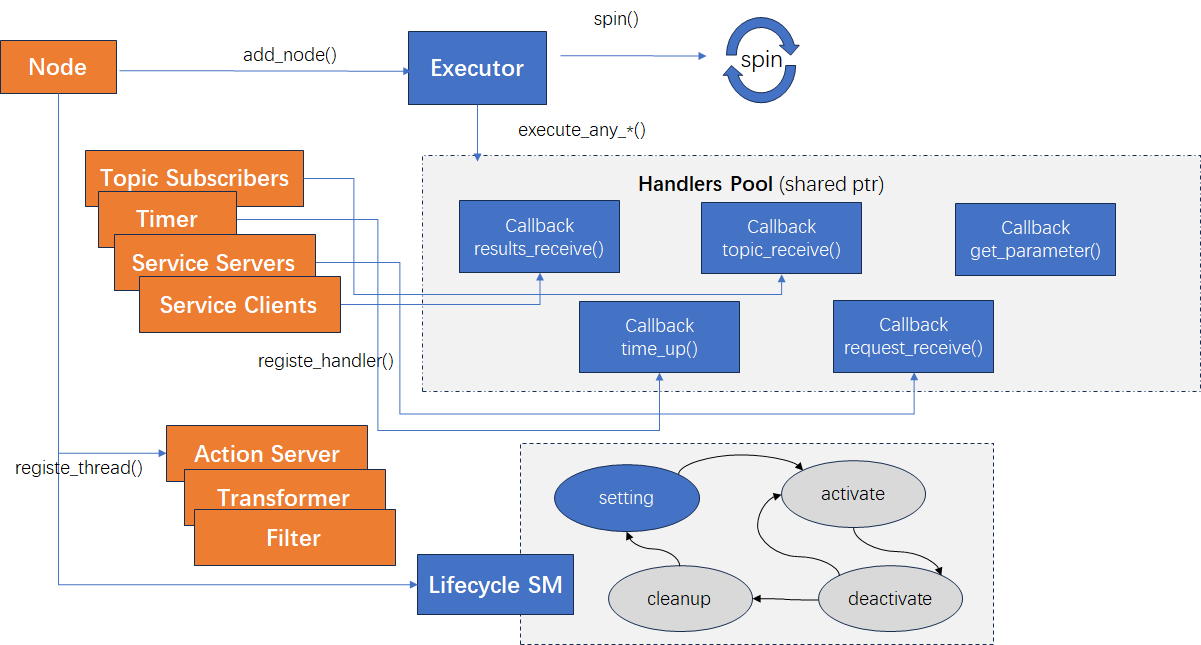
\includegraphics[width=15cm]{ros_node_setup.png}
    \caption{ROS节点内部模型, 初始阶段}
    \label{pic:rns}
\end{figure}

\textbf{ROS 节点释放}

当ROS2系统的节点将释放时,节点的生命周期状态机会从 activate 状态转换为 deactivate 状态,
此状态仅用于让节点完成必要的最后工作,如完成正在处理的数据传输或请求,然后进入非活跃状态。

紧接着,节点生命周期状态机转为 cleanup 状态,见图\ref{pic:rnc},调用 \texttt{cleanup()} 回调函数来释放节点
拥有的资源,这包括所有回调函数(callback handlers),如和话题订阅、定时器、服务等回调
函数。然后清理节点所打开的文件,断开网络连接,释放ROS2上下文,最终释放内存。

\begin{figure}[h]
    \centering
    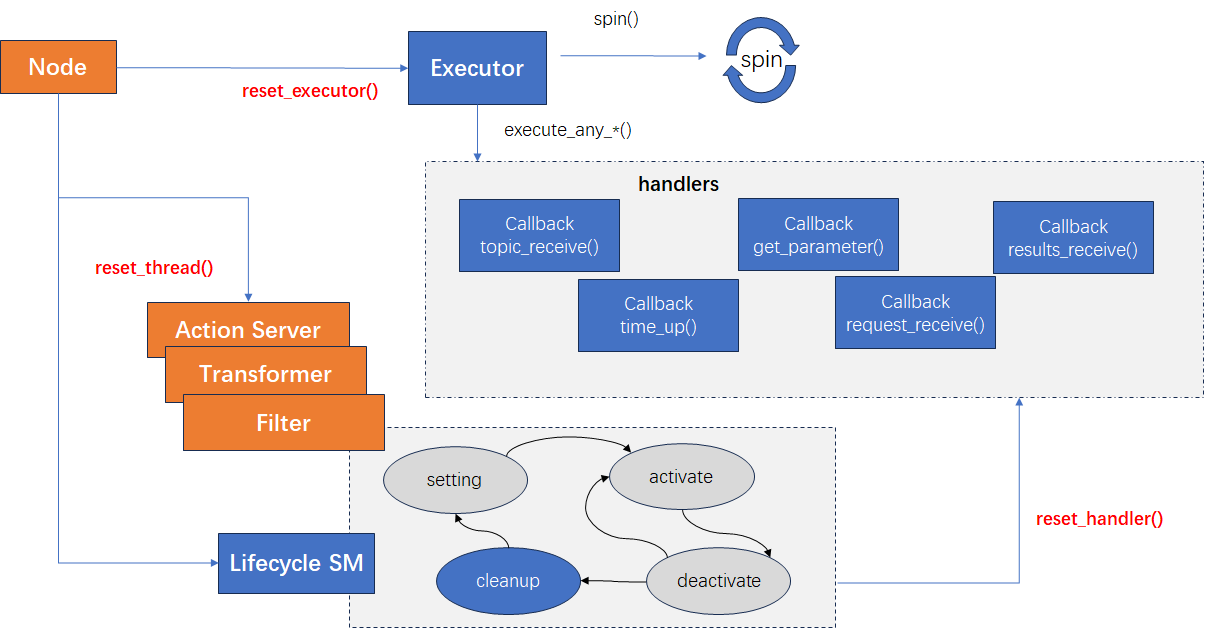
\includegraphics[width=15cm]{ros_node_cleanup.png}
    \caption{ROS节点内部模型, 释放阶段}
    \label{pic:rnc}
\end{figure}

\textbf{ROS 通信机制}

为了适应机器人系统中复杂的通信需求,ROS2设计了一套专用的通信模型。其基础为“发布、订阅“模型,支持节点间的异步数据交换。
该机制允许ROS2系统内的节点(Node)独立地发布(Publish)和订阅(Subscribe)消息,而不需要彼此之间的直接连接或相互了解。
这种设计显著提高了系统的灵活性和扩展性,因为它允许任何数量的发布者和订阅者存在于同一个话题上,从而实现了高效的多对多通信。

在ROS 2的架构中,每个节点可以根据其功能需求,声明为发布者或订阅者,类似图 \ref{pic:rmp},或同时充当这两种角色。
发布者负责生成并发布特定类型的消息到一个命名的话题上,而订阅者则监听这个话题,接收并处理传入的消息。
监听到并处理消息时,使用的是订阅该话题时传入的回调函数来自动处理,订阅者不必同步阻塞就能等待处理订阅消息。
话题本质上是一个数据通道,它通过唯一的名称标识,确保消息的传递和接收的一致性。
每个话题都与一个明确的消息类型相关联,这个消息类型使用YAML格式定义各字段的静态变量类型,从而定义了该话题传输数据的结构。

此通信机制的一个核心优点是其异步性,使得发布者和订阅者可以独立地操作,增加了处理并发消息的能力。
此外,由于发布者和订阅者之间的解耦,系统组件可以被设计得更为模块化,易于开发和维护。
例如,在自动驾驶的应用场景中,激光雷达传感器节点可以发布其测量到的数据到话题 \textbackslash scan,而负责建图和规划路径的节点
则通过订阅该话题来实时获取雷达信息,从而完成最终决策。


\begin{figure}[h]
    \centering
    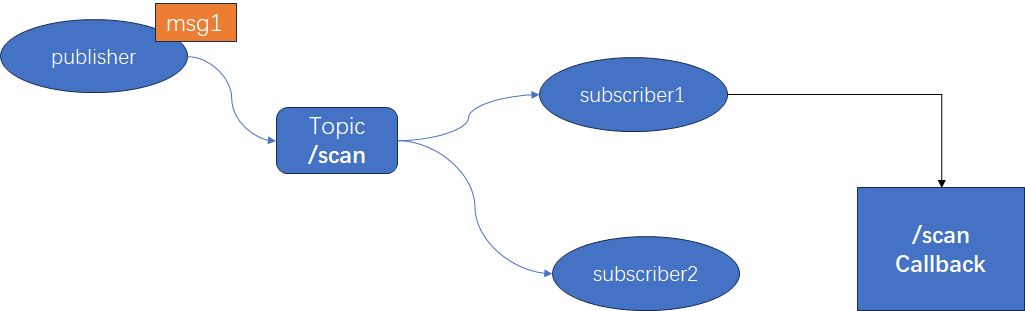
\includegraphics[width=13cm]{ros_msg_passing.png}
    \caption{ROS话题通信机制}
    \label{pic:rmp}
\end{figure}
%@author: yjw

\subsection{关键设计}
\setParDis %设置段间距为 0
%author: yjw, 2024-4-1
%\subsection{关键设计}
\subsection{系统需求分析}
\setParDis %设置段间距为 0
%@author: wkt
\begin{enumerate}
  \item 高覆盖率
  \item 高效性快速收敛
  \item 可拓展性
  \item 准确性高
\end{enumerate}
本项目核心目标是将自动模糊测试(Fuzzing)框架迁移到ROS2系统上,并且针对ROS2特性对测试效率做出改进提升。
具体而言,我们试图寻找更多可能的程序输入口,使测试覆盖的输入可能性尽可能多;尝试构造质量尽可能高的初始种子;
寻找更多反馈信息,用于监控被测程序(即ROS2节点)的内部状态,以更高效地指导对输入的变异;
尝试模拟更多ROS2执行环境,模拟程序可能遇到的各种实际情况。

\subsubsection{多维度输入}
\subsubsection{程序插桩}
\subsubsection{测试加速}


最终,给出本项目的核心框架如图\ref{pic:off}。

\begin{figure}[h]
    \centering
    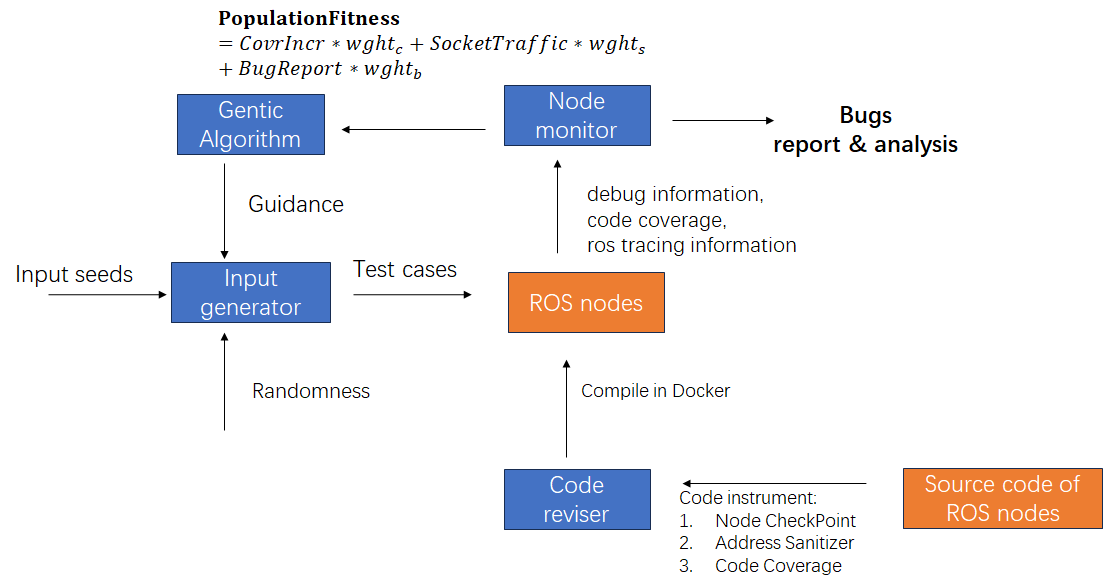
\includegraphics[width=14cm]{our_fuzz_framework.png}
    \caption{本项目实现的Fuzz框架}
    \label{pic:off}
\end{figure}

\subsubsection{测试环境}
%@author: yjw

\section{作品测试与成果分析}
\setParDis %设置段间距为 0
%@author: wkt
\subsection{测试环境介绍}
本作品在ROS2中测试了10个常见的机器人程序。根据最新版本的测试结果得到下列图表,表格1显示了这些用于测试的ROS程序的信息(源代码行数按CLOC计算{[}23{]})。为了执行机器人导航(用于移动和定位程序)和地图构建(用于移动和SLAM程序)任务,这些程序在机器人仿真框架Gazebo
11.5{[}24{]}中的虚拟机器人TurtleBot3
Waffle上执行。本测试使用的虚拟传感器包括激光雷达,里程计,2D相机和IMU(惯性测量单元)。实验运行在一台普通的x86-64台式机上,配有8个英特尔处理器和20GB物理内存。使用的操作系统为Ubuntu
20.04, ROS2版本为ROS2 Foxy。
\begin{table}[H]
	\small
	\caption{用于测试的ROS程序信息}
	\label{tb:ros_test}
	\centering
	\begin{tabular}{cccc}
		\hline  
		\textbf{类型} & \textbf{程序} & \textbf{描述} & \textbf{LOC} \\ 
		\hline  
		移动 & nav2\_bt\_navigator & ROS2导航中的BT导航模块 & 6.2K \\
		移动 & nav2\_planner & ROS2导航中的路径规划器模块 & 10.4K \\
		移动 & nav2\_recoveries & ROS2导航中的恢复模块 & 1.2K \\
		移动 & nav2\_controller & ROS2导航中的控制器模块 & 6.3K \\
		定位 & nav2\_amcl & ROS2导航中的定位模块 & 14.4K \\
		定位 & lama\_loc & 可选的定位和映射方法 & 9.5K \\
		定位 & ekf\_loc & 基于卡尔曼滤波的定位方法 & 0.8K \\
		SLAM & rtab-map & 实时RGB-D SLAM方法 & 26.1K \\
		SLAM & slam\_toolbox & 一套用于2D SLAM的工具和功能 & 15.1K \\
		SLAM & cartographer & 实时2D和3D SLAM方法 & 7.8K \\
		\hline
	\end{tabular} 
\end{table}

\subsection{测试成果与漏洞统计}
本测试运行一个通用的第三方分析工具ASan{[}20{]}和本作品来检测运行时的内存bug。每个程序都用相关的机器人任务进行24小时的测试。表格2显示了测试结果。

\begin{table}[H]
	\small
	\caption{机器人程序在ROS2模糊测试结果}
	\centering
	\begin{tabular}{ccccc}
		\hline
		\textbf{程序} & \multicolumn{2}{c}{\textbf{覆盖分支}} & \multicolumn{2}{c}{\textbf{漏洞检测}} \\
		\cline{2-5}
		& \textbf{模糊测试} & \textbf{测试样例} & \textbf{发现的漏洞} & \textbf{确认的漏洞} \\
		\hline
		nav2\_bt\_navigator & 24.3K & 17.2K & 3 & 2 \\
		nav2\_planner & 27.9K & 25.9K & 6 & 5 \\
		nav2\_recoveries & 15.8K & 16.4K & 2 & 2 \\
		nav2\_controller & 37.6K & 25.1K & 3 & 1 \\
		nav2\_amcl & 12.2K & 12.0K & 9 & 7 \\
		lama\_loc & 25.3K & 20.7K & 3 & 0 \\
		ekf\_loc & 16.2K & 5.2K & 1 & 0 \\
		rtab-map & 70.9K & 59.3K & 8 & 1 \\
		slam\_toolbox & 30.9K & 10.7K & 3 & 2 \\
		cartographer & 59.9K & 52.1K & 5 & 0 \\
		\textbf{总计} & \textbf{320.9K} & \textbf{244.5K} & \textbf{43} & \textbf{20} \\
		\hline
	\end{tabular}
\end{table}

\textbf{测试覆盖率。}为了理解本作品的测试覆盖改进,本测试还对每个ROS程序运行了24小时的官方测试用例,并收集了覆盖的代码分支的数量。得益于本作品基于ROS属性的模糊测试方法,与运行测试样例相比,本作品覆盖了测试程序中31\%的代码分支。值得一提的是,在运行官方测试用例时,本作品没有发现任何错误。

\textbf{漏洞检测。}本作品在测试程序中发现了43个真实的漏洞,没有误报。这些漏洞实际上可以使用本作品及其生成的测试用例来重现。本团队已经向相关ROS开发者报告了这些漏洞,其中20个漏洞已经得到了确认和修复,仍在等待对剩余漏洞的反馈。值得注意的是,有五个测试程序的名称包含``nav2'',它们是由ROS社区开发和维护的且广泛用于基于ROS的机器人。因此,这5个程序中已确认的17个bug受到了ROS开发者的高度关注。
\subsection{ROS漏洞实例分析}
本团队还根据发现的43个漏洞的类型进行了分类,并将结果总结在表3中。具体来说,有6个空指针解引用,5个释放后使用错误,3个缓冲区/堆栈溢出错误,11个无效指针访问和18个未捕获异常,如表格3所示。一旦这些错误被特定的输入触发,运行时故障和严重的安全问题就会在运行时发生。具体来说,空指针解引用和未捕获的异常可能导致程序崩溃,从而异常中止机器人任务;缓冲区/堆栈溢出错误、释放后使用错误和无效指针访问会导致机器人的未定义行为,并增加机器人受到恶意攻击的风险。下面将对不同种类的漏洞进行简要介绍其特点及危害。
\begin{table}[H]
	\small
	\caption{发现漏洞的种类}
	\centering
	\begin{tabular}{ccccccc}
		\hline
		\textbf{程序} & \textbf{空指针} & \textbf{释放后使用} & \textbf{溢出} & \textbf{无效指针} & \textbf{异常} & \textbf{总计} \\
		\hline
		nav2\_bt\_navigator & 1 & 0 & 0 & 0 & 2 & 3 \\
		nav2\_planner & 0 & 2 & 1 & 2 & 1 & 6 \\
		nav2\_recoveries & 0 & 2 & 0 & 0 & 0 & 2 \\
		nav2\_controller & 0 & 0 & 1 & 1 & 1 & 3 \\
		nav2\_amcl & 2 & 0 & 0 & 6 & 1 & 9 \\
		lama\_loc & 2 & 0 & 0 & 0 & 1 & 3 \\
		ekf\_loc & 0 & 0 & 0 & 0 & 1 & 1 \\
		rtab-map & 0 & 0 & 1 & 1 & 6 & 8 \\
		slam\_toolbox & 1 & 1 & 0 & 1 & 0 & 3 \\
		cartographer & 0 & 0 & 0 & 0 & 5 & 5 \\
		\textbf{总计} & \textbf{6} & \textbf{5} & \textbf{3} & \textbf{11} & \textbf{18} & \textbf{43} \\
		\hline
	\end{tabular}
\end{table}

本测试检测到的5个释放后使用漏洞是由数据竞争引起的。具体来说,一个内存对象在一个线程中被释放,但这个对象仍然在另一个线程中使用,没有同步。由于并发执行的不确定性,在正常执行中很难发现这些漏洞。一个真实含有释放后使用漏洞的代码如图表1所示

本测试检测到的这18个未捕获的异常中,有8个错误是由被测程序代码中的内部异常引起的,10个错误是由被测ROS程序使用的第三方软件库和ROS核心组件的API调用的外部异常(在c++中属于``运行时错误''类型)引起的。这个特性表明应该在ROS程序中小心地捕获和处理内部和外部异常。例如,在nav2\_bt\_navigator、nav2\_planner、nav2\_controller和nav2\_amcl中,没有捕捉到来自ROS
rclcpp组件的关于负时间间隔的四个外部异常,这可能导致程序崩溃。真实的代码案例如下图表2所示:

在ROS程序初始化过程中出现了11个bug。这些错误中有6个是由于初始化过程中对无效用户数据和不正确参数配置的错误处理引起的;还有5个漏洞是由初始化过程和消息处理之间缺少同步引起的。因此,在测试ROS程序时,应该特别注意初始化过程。

通过手工检查发现漏洞的回溯,本团队发现有7个漏洞位于被测试的ROS程序所使用的第三方库和ROS核心组件中。这些库和组件包括libopencv、fasttps、eigen、tf2和rclcpp。由于在实验中使用Asan仅仅检测被测试的ROS程序,而不是这些库或组件,因此无法找到这些漏洞的准确位置。为了解决这些问题,本作品尝试使用ASan来检测这些库和组件。但在尝试中发现,它们都不能支持ASan。即便如此,本团队在不使用ASan的情况下手动检查源代码并且成功在rclcpp中找到了一个漏洞(堆栈溢出)。目前rclcpp开发人员已经确认并修复了这个漏洞。

7个漏洞是由回调函数的并发性引起的。在ROS程序中,外部事件(如消息到达)随时会发生,并且每种事件均是由回调函数处理。由于事件可以在任何时间发生,它的回调函数可以与其他函数并发执行。因此,由于不正确的同步,回调函数中可能出现并发错误。图6(a)显示了nav2\_planner中的一个示例错误。回调函数footprint.callback可以与函数getFootprint并发执行。在footprint.callback函数中,指针footprint\_与msg在第106行一起被分配,因此由footprint\_所指向的内存会根据智能指针的功能被释放。同时,getFootprint中仍然使用这个智能指针来访问第76行中的footprint\_-\textgreater polygon,因此导致释放后使用的漏洞。{[}35{]}

11个漏洞是由错误处理问题引起的。具体来说,其中6个错误是由于对无效用户数据和错误的配置参数缺少或不正确的安全检查而引入的;另外5个错误是由于正确的安全检查后错误处理不正确而引入的。图6(b)显示了nav2\_controller中的一个示例错误。transformLaserScanToPointCloud函数可以在运行时抛出一个显式异常和一个隐式异常。在第294行只捕获显式异常,但未捕获``运行时错误''类型的隐式异常{[}36{]}。

2个漏洞是由堆栈内存问题引起的。其中一个漏洞是由在新线程中使用局部变量引起的,另一个漏洞是由过多的递归调用引起的。图6(c)显示了rtab-map中的一个示例错误。在CoreWrapper类的构造函数中,主线程的第141行定义了一个局部变量tfDelay,但是这个变量是在一个通过new
std::thread创建的新线程中的第590行被访问的。由于新线程无法访问主线程的堆栈,因此会出现堆栈溢出错误{[}37{]}。

\subsection{与同类技术对比}
本测试通过实验将本作品与两种最先进的机器人程序测试方法Ros2-fuzz{[}10{]}和ASTAA{[}38{]}进行了比较。ROS2
-fuzz是一种基于AFL{[}2{]}的自动化模糊测试方法,用于在ROS2中测试机器人程序。这种方法会对给定ROS节点中特定主题的消息进行变异。由于Ros2-fuzz是开源的,我们从源代码构建它。ASTAA是一种针对机器人程序鲁棒性测试的方法。它在ROS节点之间随机改变消息,并且还可以在运行时丢弃一些消息以模拟通信不稳定。由于ASTAA是闭源的,本团队通过修改本作品实现了一个类似ASTAA的工具,只允许传感器消息的数据突变和随机丢弃消息,而不使用程序反馈。

在实验中,我们在表1中选择了5个名称包含``nav2''的程序,并运行Ros2-fuzz、ASTAAlike工具和本作品对这些程序进行了24小时的机器人导航任务测试。表4显示了比较结果,其中包括覆盖的代码分支和发现的漏洞。
\begin{table}[H]
	\small
	\caption{不同测试方法的漏洞检测结果}
	\centering
	\begin{tabular}{ccccccc}
		\hline
		\multirow{2}{*}{\textbf{程序}} & \multicolumn{2}{c}{\textbf{Ros2-fuzz}} & \multicolumn{2}{c}{\textbf{ASTAA-like}} & \multicolumn{2}{c}{\textbf{本作品}} \\
		\cline{2-7}
		& \textbf{分支} & \textbf{发现漏洞数} & \textbf{分支} & \textbf{发现漏洞数} & \textbf{分支} & \textbf{发现漏洞数} \\
		\hline
		nav2\_bt\_navigator & 1.8K & 0 & 23.7K & 1 & 24.3K & 3 \\
		nav2\_planner & 1.6K & 0 & 26.4K & 2 & 27.9K & 6 \\
		nav2\_recoveries & 4.8K & 0 & 15.1K & 1 & 15.8K & 2 \\
		nav2\_controller & 3.1K & 0 & 35.2K & 3 & 37.6K & 3 \\
		nav2\_amcl & 0.7K & 0 & 11.9K & 2 & 12.2K & 9 \\
		\textbf{总计} & \textbf{12.0K} & \textbf{0} & \textbf{112.3K} & \textbf{9} & \textbf{117.8K} & \textbf{23} \\
		\hline
	\end{tabular}
\end{table}
本作品发现了Ros2-fuzz和ASTAA-like的工具发现的所有9个漏洞,并且它还发现了这些方法遗漏的14个漏洞,且具有更高的代码覆盖率。实际上,Ros2-fuzz和ASTAA仅生成关于ROS节点之间消息的测试用例,因此在模糊测试期间没有涉及处理不同用户数据和配置参数的大量代码。相比之下,本作品从多个维度(包括用户数据、配置参数和传感器消息)生成测试用例,因此本作品覆盖了Ros2-fuzz和ASTAA遗漏的更多代码。此外,本作品使用分布式分支覆盖更有效地指导多个ROS节点的测试用例生成,并使用三种常见模式执行时间突变(ASTAA只考虑其中一种模式,即消息丢弃),以更有效地覆盖有关时间特征的代码。由于这些原因,在实验中,本作品比Ros2-fuzz和类ASTAA-like的工具产生更好的结果。

通过分析被覆盖分支随着测试时间的增长,观察到随着时间的推移,这三种工具覆盖的新代码分支越来越少。这是因为许多代码分支已经被模糊测试期间由早期突变生成的测试用例所覆盖。即便如此,本团队观察到在后面的测试中,由于本项目的多维生成方法、分布式分支覆盖和时间突变策略,本作品覆盖了更多的新代码分支。

本作品也适用于在ROS1中测试机器人程序。因此,本团队使用本作品和ASan来测试了ROS1中三个常见的机器人程序,包括move\_base
{[}39{]}, nav1\_
amcl{[}40{]}和hector\_mapping{[}41{]}。对于机器人导航任务,本团队运行move\_base和nav1\_amcl,然后运行move\_base和hector\_mapping来完成地图建立任务。本团队对每个程序及其相关任务测试24小时。与第IV-A节类似,同时还运行每个程序的官方测试样例24小时,以验证本作品的测试覆盖改进。表5显示了测试结果。
\begin{table}[H]
	\small
	\caption{ROS1中机器人程序测试结果}
	\centering
	\begin{tabular}{cccccc}
		\hline
		\multirow{2}{*}{\textbf{程序}} & \multicolumn{2}{c}{\textbf{覆盖分支}} & \multicolumn{3}{c}{\textbf{发现的漏洞}} \\
		\cline{2-6}
		& \textbf{模糊测试} & \textbf{测试套件} & \textbf{无效指针} & \textbf{异常} & \textbf{总计} \\
		\hline
		move\_base & 36.4K & 31.9K & 0 & 2 & 2 \\
		navl\_amcl & 12.5K & 10.9K & 2 & 2 & 4 \\
		hector\_mapping & 13.1K & 11.5K & 0 & 0 & 0 \\
		\textbf{总计} & \textbf{62.0K} & \textbf{54.3K} & \textbf{2} & \textbf{4} & \textbf{6} \\
		\hline
	\end{tabular}
\end{table}

与运行测试样例相比,本作品在测试程序中覆盖了14\%的代码分支,这得益于我们基于ROS属性的模糊测试方法。值得注意的是,在运行官方测试样例时,我们没有发现任何错误。由于测试覆盖率的提高,本作品发现了6个真正的错误,没有误报,包括2个无效指针访问和4个未捕获的异常。本团队已经向相关ROS开发人员报告了这些报告,但尚未收到任何回应。实际上,这三个测试程序的github存储库已经很长时间没有更新了。
\subsection{测试环境介绍}
\setParDis %设置段间距为 0
\subsection{测试成果与漏洞统计}
\setParDis %设置段间距为 0
\subsection{ROS漏洞实例分析}
\setParDis %设置段间距为 0
相关讨论可见GitHub问题 \href{https://github.com/ros-planning/navigation2/issues/4177}{Issue\#4177},提出了ROS 2通信机制中的一个潜在的缓冲区溢出问题。

\begin{lstlisting}[language=]
ros2 topic pub /map nav_msgs/msg/OccupancyGrid "
header:
  stamp:
    sec: 0
    nanosec: 0
  frame_id: map
info:
  map_load_time:
    sec: 0
    nanosec: 0
  resolution: 0.05000000074505806
  width: 2
  height: 2
  origin:
    position:
      x: -10.0
      y: -10.0
      z: 0.0
    orientation:
      x: 0.0
      y: 0.0
      z: 0.0
      w: 1.0
data: [-1, ] " <- buffer overflow
\end{lstlisting}

当\texttt{size\_x\_}和\texttt{size\_y\_}大于数组\texttt{data}大小时,就会导致访问越界(SEGV)。初始化时和接收到\texttt{/map}消息时触发此问题,展示了危险的代码实践。

\begin{lstlisting}[language=cpp]
// create the costmap
costmap_ = new unsigned char[size_x_ * size_y_];

for (unsigned int it = 0; it < size_x_ * size_y_; it++) {
  data = map.data[it]; // <- SEGV
  if (data == nav2_util::OCC_GRID_UNKNOWN) {
    costmap_[it] = NO_INFORMATION;
  } else {
    ...
  }
}
\end{lstlisting}

相关问题和解决方案还包括GitHub \href{https://github.com/ros-planning/navigation2/pull/3958}{PR\#3972}, \href{https://github.com/ros-planning/navigation2/pull/3958}{PR\#3958}, \href{https://github.com/ros-planning/navigation2/issues/3940}{Issue\#3940}, 揭示了并发bug,并通过两个PullRequest得到解决,节省了大量不必要的检查。

最后,讨论了ROS 2节点退出机制可能出现的并发问题,详见 \href{https://github.com/ros-planning/navigation2/issues/4175}{Issue\#4175}, \href{https://github.com/ros-planning/navigation2/pull/4180}{PR\#4180}, \href{https://github.com/ros-planning/navigation2/issues/4166}{Issue\#4166}, \href{https://github.com/ros-planning/navigation2/pull/4176}{Pull\#4176}, 和 \href{https://github.com/ros2/rclcpp/issues/2447}{RclCpp Issue\#2447}。

\subsection{实例分析}
\setParDis %设置段间距为 0
\subsection{与同类技术对比}
\setParDis %设置段间距为 0

\section{创新型说明与前景分析}
\setParDis %设置段间距为 0
%@author: jfb
\subsection{创新性说明}
\setParDis %设置段间距为 0
\begin{enumerate}
  \item 创新地将模糊测试技术迁移
  \item 创新测试方法,高效性
\end{enumerate}

\subsection{前景分析}
\setParDis %设置段间距为 0
\begin{enumerate}
  \item 创新维度
  \item 团队维度
  \item 商业维度
  \item 就业维度
  \item 社会服务
\end{enumerate}

\section*{结论}% section*生成无标号章节
\addcontentsline{toc}{section}{结论} % 将无标号章节添加至目录
%@author: jfb
傻逼冯如杯

%注意: 文件大小不超过5M。%

\end{spacing}
%%%%%%%%%%%%%%%%%%%%引用部分
\newpage

% XSP 2023/3/16: bib支持不全,暂时改为手动
\section*{参考文献} % section*生成无标号章节题目
\addcontentsline{toc}{section}{参考文献} % 将无标号章节添加至目录
% 著作: [序号]作者.书名[标识码].出版地:出版社,出版年.
[1]张志建.严复思想研究[M].桂林:广西师范大学出版社,1989. 

% 译著: [序号]国名或地区(用圆括号)原作者.书名[标识码].译者.出版地:出版社,出版年.
[2](英)霭理士.性心理学[M].潘光旦译.北京:商务印书馆,1997.

% 古典文献 文史古籍类引文后加序号,再加圆括号,内加注书名、篇名

% 论文集: [序号]编者.书名[标识码].出版地:出版社,出版年.
[3]伍蠡甫.西方论文选(下册)[C].上海:上海译文出版社,1979.

% 期刊文章: [序号]作者.篇名[标识码].刊名,年,(期).
[4]叶朗.《红楼梦》的意蕴[J].北京大学学报(哲学社会科学版),1989,(2)

% 报纸文章: [序号]作者.篇名[标识码].报纸名,出版日期(版次)
[5]谢希德.创造学习的新思路[N].人民日报,1998-12-25(10)

% 外文文献: 要求外文文献所表达的信息和中文文献一样多,但文献类型标识码可以不标出。
[6]Mansfeld, R.S. \& Busse. \textit{T.V. The Psychology of creativity and discovery}, Chinago:
NelsonHall, 1981




% \begingroup
% \setstretch{2.0}    %行距2
% \setlength{\bibsep}{0pt}    %段前段后0
% \begin{adjustwidth}{0.42cm}{0.42cm} %左右缩进0.42cm
% \bibliography{references}
% \end{adjustwidth}
% \endgroup

\end{document}
